\chapter{A Comunicação \textit{Modbus}}
\label{c:a_comunicacao_modbus}
% ---
\section{O protocolo \textit{Modbus}}

O \textit{Modbus} é um protocolo amplamente utilizado no setor de automação industrial, principalmente por sua simplicidade e facilidade de implementação. Este protocolo permite que seja usada uma mesma linguagem de comunicação em diversos padrões de meio físico, variando a velocidade de comunicação, quantidade de dispositivos suportados na rede bem como o comprimento máximo da mesma, fazendo assim com que cada tipo de estrutura física seja adequada à um cenário de projeto, justificando com isso a sua ampla utilização.

Os padrões de meio físico definem o modo de comunicação através do qual os dados serão transmitidos entre o mestre e seus escravos. O protocolo pode ser utilizado por uma aplicação por um meio serial ou através de conexões TCP (\textit{Ethernet}), tendo por exemplo os padrões RS-232,RS-4222 e RS-485 para a comunicação serial e o modbus TCP para a comunicação através de endereços IP para cada dispositivo \cite{dutertre2007formal}.

O padrão RS-232 (Recommended Standard 232) ou EIA-232 (Electronic Industries Alliance 232) é utilizado apenas quando se possui apenas dois dispositivos na rede, formando a chamada comunicação ponto a ponto,  onde no protocolo \textit{Modbus} representa o mestre e o escravo. Este padrão alcança velocidades em uma média de 115 Kbps, podendo ultrapassar este valor em um pequeno percentual, dependendo da qualidade estrutural da rede. A distância máxima entre o escravo e o mestre da rede é de aproximadamente 30 metros.

O padrão RS-485 (Recommended Standard 485) ou EIA-485 (Electronic Industries Alliance 485) é um dos padrões mais utilizados industrialmente, dentre os outros com comunicação serial. Uma das principais vantagens em relação ao RS-232 é que a comunicação mestre escravo não fica limitada a apenas dois dispositivos, podendo estabelecer uma comunicação de até 32 dispositivos por barramento na rede. Além disso a sua velocidade de conexão é bem superior aos 115 Kbps descritos no parágrafo anterior, podendo chegar à 50Mbps, dependo do comprimento da rede, sendo que quanto maior for, menor será a velocidade de comunicação sendo que nesse caso o alcance máximo da rede é por volta de 1200 metros.


Já o protocolo TCP, como o próprio nome sugere, utiliza TCP como camada de comunicação, porém tentando manter uma compatibilidade com o protocolo serial Modbus. Para possibilitar a diferenciação de cada escravo é atribuído um endereço IP para o dispositivo através do qual o mesmo será identificado na rede, além disso o protocolo \textit{Modbus} TCP utiliza por padrão um número de porta IP específico (502) para a comunicação. O Modbus TCP possui uma vantagem econômica devido à maior facilidade de implantação por conta da ampla disponibilidade de redes compatíveis com a comunicação TCP, porém esta alta disponibilidade traz consigo uma preocupação maior em relação à segurança dos dados transmitidos na rede. 


\section{Formato de uma mensagem \textit{Modbus}}

A estrutura de uma mensagem transmitida com base no protocolo \textit{Modbus} RTU é definida na figura \ref{fig:Modbus}, porém podemos utilizar a mesma como base para o modelo ASCII diferenciando-se por um caractere inicial ":" (ASCII 0x3Ah) 
e um CRLF (\textit{Carriage Return and Line Feed}) representado em ASCII por 0x0Dh + 0x0Ah ao final da mensagem:
\newline

\begin{figure}[h]
\caption{Estrutura da Mensagem \textit{Modbus}}
\centering
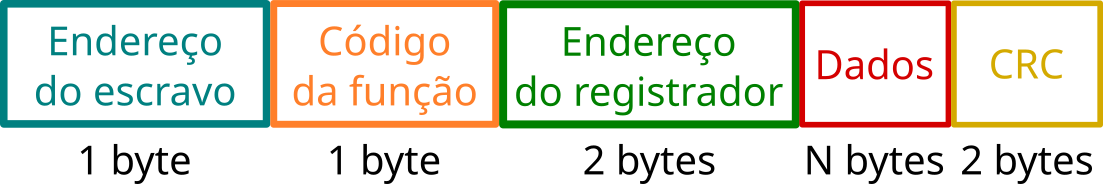
\includegraphics[width=1.0\textwidth,height=1.0\textheight,keepaspectratio]{imagens/mensagem-modbus.png}
\caption*{Fonte: Próprio Autor}
\label{fig:Modbus}
\end{figure}

\subsection{Endereçamento}

No caso da comunicação serial a mensagem conterá inicialmente 1 byte com o endereçamento do dispositivo de destino da mensagem, podem ir de 1 a 256. Já para a comunicação TCP o início da mensagem conterá um cabeçalho que basicamente é composto pelo endereçamento IP do dispositivo de destino da mensagem.

\subsection{Função}

Neste campo de 1 byte o dispositivo mestre indicará qual o tipo de serviço ou função que será solicitada ao escravo. No protocolo \textit{Modbus}, cada função é utilizada para acessar um tipo específico de dado. Algumas dessas funções estão descritas na tabela \ref{tab:tabela_funcoes_modbus} para efeito de exemplificação.


\begin{table}[H]
\centering
\caption{Lista de Algumas Funções do Protocolo Modbus}
\label{tab:tabela_funcoes_modbus}
\begin{tabular}{| l | m{11cm} |}
\hline
\textbf{Código da Função} & {\center \textbf{Descrição}} \\ [10pt]
\hline
0x01 & Leitura de bloco de bits do tipo coil (saída discreta) \\ 
\hline
0x02 & Leitura de bloco de bits do tipo entradas discretas \\ 
\hline
0x03 & Leitura de um número variável de registros retentivos (saídas analógicas ou memórias) \\ 
\hline
0x04 & Leitura de um número variável de registros de entrada (entradas analógicas)\\ 
\hline
0x05 & Escrita em um único bit do tipo coil (saída discreta) \\ 
\hline
0x06 & Escrita em um único registrador (altera o estado de uma saída analógica)\\ 
\hline
0x07 & Leitura do conteúdo de 8 estados de exceção (registro de erros) \\ 
\hline
0x08 & Execução de uma série de testes para verificação da comunicação e erros internos\\ 
\hline
\end{tabular}
\end{table}

\subsection{Dados}

Este campo possui um tamanho em bytes variável dependendo do conteúdo de retorno da mensagem solicitada pelo mestre através do código da função passada ou da informação que será registrada no escravo, sendo que esta mensagem será inserida no corpo da mensagem pelo mestre.

\subsection{CRC}

Para os protocolos com comunicação serial, ao final da mensagem existirão 2 bytes contendo uma mensagem de verificação de erros na transmissão da mesma, preenchidos por um algoritmo de CRC (\textit{Cyclic Redundancy Check}). Essa mensagem garantirá a consistência do envio completo da mensagem.
Já para o protocolo de comunicação TCP, os bytes finais de verificação de erro já não se fazem necessários.


